
%%%%%%%%%%%%%%%%%%%% book.tex %%%%%%%%%%%%%%%%%%%%%%%%%%%%%
%
% sample root file for the chapters of your "monograph"
%
% Use this file as a template for your own input.
%
%%%%%%%%%%%%%%%% Springer-Verlag %%%%%%%%%%%%%%%%%%%%%%%%%%


% RECOMMENDED %%%%%%%%%%%%%%%%%%%%%%%%%%%%%%%%%%%%%%%%%%%%%%%%%%%
\documentclass[graybox,envcountchap,sectrefs]{svmono}

% choose options for [] as required from the list
% in the Reference Guide

\usepackage{color}   %May be necessary if you want to color links
\usepackage{hyperref}
\hypersetup{
    colorlinks=false, %set true if you want colored links
    linktoc=all,     %set to all if you want both sections and subsections linked
    linkcolor=red,  %choose some color if you want links to stand out
    urlcolor=blue,
    citecolor=green,
}
\usepackage{mathptmx}
\usepackage{helvet}
\usepackage{courier}
\usepackage{type1cm}         
\usepackage{makeidx}         % allows index generation
\usepackage{graphicx}        % standard LaTeX graphics tool
                             % when including figure files
\usepackage{multicol}        % used for the two-column index
\usepackage[bottom]{footmisc}% places footnotes at page bottom

\usepackage{newtxtext}       % 
\usepackage[varvw]{newtxmath}       % selects Times Roman as basic font

% see the list of further useful packages
% in the Reference Guide

\makeindex            % used for the subject index
                       % please use the style svind.ist with
                       % your makeindex program

%%%%%%%%%%%%%%%%%%%%%%%%%%%%%%%%%%%%%%%%%%%%%%%%%%%%%%%%%%%%%%%%%%%%%

\begin{document}


\title{\center{The Elements} \\ \center{of Integration and} \\ \center{Lebesgue Measure}}
\author{\center{BARTLE}}
\subtitle{\center{\TeX\;typesetting by Ali Darijani}}

\maketitle

\frontmatter%%%%%%%%%%%%%%%%%%%%%%%%%%%%%%%%%%%%%%%%%%%%%%%%%%%%%%




\tableofcontents
% %%%%%%%%%%%%%%%%%%%%%%foreword.tex%%%%%%%%%%%%%%%%%%%%%%%%%%%%%%%%%
% sample foreword
%
% Use this file as a template for your own input.
%
%%%%%%%%%%%%%%%%%%%%%%%% Springer %%%%%%%%%%%%%%%%%%%%%%%%%%
\Extrachap{Foreward}
%% Please have the foreword written here
Surely, Antoni Zygmund's \textit{Trigonometric Series} has been, and continues to be, one of the most influential 
books in the history of mathematical analysis.Therefore, the current printing, which ensures the future availability of 
this work to the mathematical public is an event of major importance. Its tremendous longevity is a testimony 
to its depth and clarity. Generations of mathematicians from Hardy and Littlewood to recent classes of graduate 
students specializing in analysis have viewed \textit{Trigonometric Series} with enormous admiration and have 
profited greatly from reading it. In light of the importance of Antoni Zygmund as a mathematician and of the 
impact of \textit{Trigonometric Series}, it is only fitting that a brief discussion of his life and mathematics accompany 
the present volume, and this is what I have attempted to give here\footnote[1]{I have been fortunate to have a number of 
excelent references to consult regarding the life of Antoni Zygmund. The reader interested in aditional material 
may consult the references in the bibliography to this Foreword.}. I can only hope that it provides at least 
a small glimpse into the story of this masterpiece and of the man who produced it.\\
\indent Antoni Zygmund was born on December 26, 1900 in Warsaw, Poland. His parents had received relatively 
little education, and were of modest means, so his background was far less privileged than that of the vast majority 
of his colleagues. Zygmund attended school through the middle of high school in Warsaw. When World War I broke 
out, his family was evacuated to Poltava in the Ukraine, where he continued his studies. When the war ended 
in 1918, his family returned to Warsaw, where he completed pre collegiate work, and entered Warsaw University. 
Zygmund's main interest throughout his childhood was astronomy, but at Warsaw University at that time there 
were not sufficient courses offered in that subject to make it realistic as a specialization, and so 
Zygmund turned instead toward another of his interests, mathematics.\\
\indent  There were a number of excelent mathematicians and teachers who profoundly influenced Zygmund during 
this period. The greatest impact came from Aleksander Rajchman and Stanislaw Saks. Rajchman was a junior 
faculty member who was an expert on Riemann's theory of trigonometric series, and Saks a felow student 
who was a few years his senior. From Rajchman, he learned much of the Riemann theory, and his doctoral thesis 
in 1923 was on this subject. Zygmund became an active colaborator with both Rajchman and Saks, publishing 
a number of important articles with each of them. In adition, Saks and Zygmund produced \textit{Analytic Functions}, 
one of the classic texts on complex analysis.\\
\indent One year prior to his PhD, Zygmund was appointed to an instructorship at the Warsaw Polytechnical 
School, and, in 1926, he was appointed Privatdozent at the University of Warsaw. He was awarded a Rockefeller fellowship, 
which he used to travel to England for the academic year of 1929-30 and visit G.H. Hardy at Cambridge 
for the first half of the year, and J.E. Litlewod at Oxford for the second half. This experience had a tremendous 
impact on the young Zygmund. Not only did he work with two of the greatest analysts of the time, but while in 
England, he also met another young mathematician, R.E.A.C. Paley, a student of Littlewod, with whom he had 
an extended and very fruitful collaboration. When he returned to Poland in 1930, Zygmund moved to Wilno where 
he took a chair in mathematics at the Stefan Batory University. It was here that Zygmund's talent and quiet charismasa 
as a teacher of advanced mathematics began to have a very major impact on the field. In the fall of 1930, 
Zygmund met a new student at the University, Jozef Marcinkiewicz. Marcinkiewicz was recognized, even when he 
was a student, as being tremendously talented, with the potential to become a serious mathematician. In the 
following year, which was only the second at Stefan Batory for both teacher and student, Zygmund decided to 
offer a course on trigonometric series preceded by lectures on Lebesgue integration. Marcinkiewicz attended 
this course, and thus began his association with Zygmund. It took just three years for Marcinkiewicz to obtain 
his masters degree, with a thesis that contained the highly non-trivial result that it is possible for 
a continuous periodic function to have interpolating polynomials corresponding to equidistant nodal points 
diverging almost everywhere. This result was elaborated to form his PhD thesis in 1935, and in 1937 Marcinkicwicz 
became Dozent in Wilno. In the period from 1935 to 1939, a collaboration between Marcinkiewicz and Zygmund 
developed that was incredibly successful. Though of relatively short duration, their work opened a number of 
new directions, and in a sense set the stage for the theory of singular integrals which would be Antoni Zygmund's 
greatest contribution.\\
\indent The years in which Zygmund was a young profesor in Wilno, though very productive mathematically, 
were not easy ones. This was due in large part to Zygmund's courageous opposition to the bigotry which was 
all to common around him, and which was supported by the higher authorities. An example of this was his 
strong dislike of anti-Semitic policies with in his university. At one time,for instance, student organizations, 
somewhat analogous to modern day fraternities, were sufficiently influential to mandate that all Jewish 
students must sit on the left side of each classroom during lectures. For Zygmund, this was completely unacceptable 
and in response, he decided to move his classes from the larger hals to small mathematics department seminar rooms 
where there were only long tables in a central arrangement, and hence no seats at the left or right of the 
room. Another illustration of Zygmund's sensitivity to issues of social justice had to do with is university's 
requirement that all student associations have faculty members as their academic sponsors. Zygmund 
regularly sponsored associations which were not in favor with the Polish government. These unpopular moves on 
Zygmund's part did not go unnoticed, and in the year 1931, as part of the political purges of the universities by 
the government, Zygmund was dismissed from his professorship. This immediately brought extremely strong reaction 
from some of the most distinguished mathematicians in Europe.From Lebesgue in France, and  from Hardy and 
Littlewod in England came formal written protests which resulted in Zygmund's reinstatement as professor. 
It is therefore an important aspect of Zygmund's life that, in a very real sense, he was a crusader for human 
rights well before this was fashionable.\\
\indent Among the many remarkable contributions of the Wilno period is the writing of the first version of 
this book, published in Warsaw under the title \textit{Trigonometrical Series}. This was Zygmund's first book, 
and it was published as volume \romannumeral 14 of the series Monografie Matematyczne. This is the same series in which the 
celebrated book \textit{Theorie des Operations Lineaires} by S. Banach appears as volume .The tremendous success 
of \textit{Trigonometrical Series} led to its expansion and revision in to a second edition, published in 1959 
by Cambridge University Press, and then to no fewer than six reprinted versions after that.\\
\indent The time in Wilno which featured the rapid achievement of success came to a sudden end in September 1939 
as World War 2 erupted. At that time, both Zygmund and Marcinkicwicz were mobilized as reserve oficers in 
the Polish army, and, as a result of the temporary ``friendship" between Germany and Russia, Poland was partitioned. 
The Soviets were given control of much of the country, including the part containing Wilno, and they preceded to round up 
and execute many of the Polish officer corps in the Katyn Forest massacre. Most likely, this is how Marcinkiewicz 
perished. Almost by a miracle, Zygmund was able to return to his family and escape with them to the United States, 
but his loss was absolutely devastating. His principal collaborators up to that time besides Marcinkicwicz had 
been Saks, Rajchmanand, Paley. Both Saks and Rajchman were murdered by the Nazis, and Paley had died in a 
tragic accident in 1933. These loses were not just mathematical. Zygmund had been extremely close to each of 
them, and so the war period must surely have been one of the most difficult of his life.\\
\indent By 1939, Zygmund had an international reputation, and many friends all over the mathematical world. It was due 
to the efforts of some of these friends, such as Jacob Tamarkin, Jerzy Neyman and Norbert Wiener, that Zygmund was 
able to emigrate to the United States in 1940. During the time immediately prior to the United States entering 
in to the war, there were very few jobs available to mathematicians. Nevertheless, after teaching for a 
semester at MIT, Zygmund was offered and accepted a position at Mount Holyoke College in central Massachusetts. 
A few years later, other offers followed. In 1945, Zygmund became a professor at the University of Pennsylvania, 
and then, in 1947, he was offered a professorship at the University of Chicago.\\
\indent The University of Chicago mathematics department, which had had a tradition of great strength, 
had experienced a period of decline prior to World War 2. During the war, the president of the university, 
Robert Maynard Hutchins, brought the Manhatan project to the campus, and with it camea number of outstanding 
scientists, such as Enrico Fermi. Hutchins then decided to make it a priority to strengthen the mathematics 
department in order to match the high quality of physical science apointments that had been made. To this end, 
a new chairman, Marshal Stone, was brought to the university and asked to bring about this improvement. 
The result was some thing phenomenal. In the period just after the war, Stone was able to asemble one of the 
best mathematics departments in history. At this time, the faculty of mathematics included such members as A.A. Albert, 
S.S. Chern, L. Graves, P. Halmos, I. Kaplansky, S. MacLane, I. Segal, E. Spanier, M. Stone, A. Weil and A. Zygmund. 
Together with this influx of great mathematicians there came a corresponding influx of brilliant students.\\
\indent The combination of such a strong mathematician and teacher as Zygmund with the unusualy rich mathematical 
environment of the University of Chicago produced a golden period of creativity and of supervision of exceptional 
students for Zygmund that was the crowning achievement of his life's work. In several cases, the route of 
outstanding students to Chicago was not totally straightforward, and the most famous case was that of Alberto P. Calderon. 
The story of the means by which Calderon came to Chicago is legendary. The following, taken from the introduction 
to the book, \textit{Essays in Honor of Alberto P.Calderon}~\cite{albertohonor} tells the story beautifuly:\\
\noindent In the years imediately after World War 2, the U.S. Department of State had a very active visitors 
program that sent prominent scientists to Latin America. Thus, Adrian Albert, Marshal Stone, and George Birkhoff 
visited Buenos Aires, and Gonzalez Dominguez arranged through them the visit of Zygmund, whose work on Fourier Series 
he much admired. At the Institute of Mathematics, Zygmund gave a two-month seminar on topics in analysis, 
based on his book. This seminar was atended by Gonzalez Dominguez, Calderon, Mischa Cotlar, and three other 
young Argentine mathematicians. Each of the participants had to discus a portion of the text. Calderon's 
assignment was to present the Marcel Riesz theorem on the continuity of the Hilbert transform in $L^p$. 
According to Cotlar's vivid recollection of the event, Calderon's exposition was entirely aceptable to the 
junior audience, but not to Zygmuncl, who appeared agitated and grimaced all the time. Finally, he interrupted 
Calderon abruptly to ask where had read the material he was presenting, and a bewildered Calderon answered 
that he had read it in Zygmund's book. Zygmund vehemently informed the audience that this was not the proof 
in his book, and after the lecture took Calderon aside and quized him about the new short and elegant proof. 
Calderon confessed that he had first tried to prove the theorem by himself, and then thinking he could not 
do it, had read the begining of the proof in the book; but after the first couple of lines, instead of turning 
the page, had figured out how the proof would finish. In fact, he had found himself an elegant new proof of 
the Riesz Theorem! Zygmund imediately recognized Calderon's power and then and there decided to invite him to 
Chicago to study wit him.\\
\indent This anecdote illustrates one of Calderon's main characteristics\dots \\ \\
\noindent The anecdote above also illustrates one of Zygmund's main characteristics: His tremendous desire to 
work with people of the greatest mathematic ability, and his absolute devotion to those people. Calderon 
came to the University of Chicago in 1949 on a Rockefeller fellowship, and only one year later received his 
PhD there under Zygmund's supervision. The thesis consisted of three research papers, each of which was a major 
work. In particular, among the results of the thesis was one of the greatest importance, concerning the boundary 
behavior of harmonic functions of several variables, which represented a crucial step in carying out the real 
variable program of Zygmund which will be described below. The collaboration betwen Calderon and Zygmund which 
followed was certainly one of the greatest in the history of modern analysis, and created a theory, the so-called 
Calderon-Zygmund Theory of Singular Integrals, that not only allowed for the extension of much of classical 
Fourier analysis from one to several dimensions,but played a fundamental role in the development of the theories 
of partial differential equations and geometry as well.\\
\indent More than simply creating a new powerful mathematical theory at Chicago, Zygmund created a school, 
the Chicago School of Analysis, which was to have an enormous impact on the subject in the next five decades, 
and promises to continue to do so in the future. After Calderon, there came other students who worked with 
Zygmund and who individually made historic contributions to mathematics. In 1955, Elias M. Stein received his 
doctorate under Zygmund, and, as is well known, by his brilliant research and teaching went on to establish 
a great school at Princeton. A bit later, other remarkable students finished their thesis work with Zygmund, 
including Paul Cohen and Guido and Mary Weiss. Taking into account the generations of students whose mathematical 
ancestry is traceable back to Zygmund, it is hard to imagine what mathematical analysis would be like without 
their collective contribution.\\
\indent At Chicago, Zygmund had a total of thirty-five students. His collected works include some 215 articles. 
Zygmund received many formal honors in his lifetime. He was a recipient of the Steele Prize of the American 
Mathematical Society, as well as the National Medal of Science, the highest award given by the United States 
government in recognition of scientific achievement. In addition, he was given membership of a number of academics, 
including the National Academy of Sciences and the American Academy for Arts and Sciences(USA), the Polish 
Academy of Sciences, the Argentina Academy of Sciences, Royal Academy of Sciences of Spain, and the Academy, 
of Arts and Sciences of Palermo, Italy. Zygmund also held honorary degrees from Washington University, the 
University of Torun, Poland, the University of Paris and the University of Uppsala, Sweden.\\
\indent After a very long and productive life in which he published his last, research article at the age of 
79, he finally slowed considerably, and, after a long illness, died at the age of 91. Few mathematicians have 
provided such a striking and wonderful counter example to G.H. Hardy's view on the rapidity of loss of creativity 
that mathematicians suffer with age.\\
\indent Zygmund's life events and his mathematics, particularly that covered in the present volume, are heavily 
intertwined. In what follows, I would like to discuss this mathematics in the context of the historical perspective 
considered above.\\
\indent continued:-)






\vspace{\baselineskip}
\begin{flushright}\noindent
University of Chicago, \hfill {\it Robert A. Fefferman}\\
\end{flushright}



%%%%%%%%%%%%%%%%%%%%%%preface.tex%%%%%%%%%%%%%%%%%%%%%%%%%%%%%%%%%%%%%%%%%
% sample preface
%
% Use this file as a template for your own input.
%
%%%%%%%%%%%%%%%%%%%%%%%% Springer %%%%%%%%%%%%%%%%%%%%%%%%%%
% \Extrachap{Preface}
\preface

%% Please write your preface here
\indent This book consists of two separate, but closely related, parts. The first part (Chapters $1-10$) is subtitled 
\textit{The Elements of Integration;} the second part (Chapters $11-17$) is subtitled \textit{The Elements of Lebesgue measure.} 
It is possible to read these two parts in either order, with only a bit of repetition.\\
\indent The Elements of Integration is essentially a corrected reprint of a book with that title, originally published in 1966, 
designed to present the chief results of the Lebesgue theory of integration to a reader having only a modest mathematical background. 
This book developed from my lectures at the University of Illinois, Urbana-Champaign, and it was subsequently used there and elsewhere 
with considerable success. Its only prerequisites are a understanding of elementary real analysis and the ability to comprehend ``$\varepsilon - \delta$ 
arguments''. We suppose that the reader has some familiarity with the Riemann integral so that it is not necessary to provide 
motivation and detailed discussion, but we do not assume that the reader has a mastery of the subtleties of that theory. A solid 
course in ``advanced calculus'', an understanding of the first third of my book \textit{The Elements of Real Analysis,} or of most 
of my book \textit{Introduction to Real Analysis} with D. R. Sherbert provides an adequate background. In preparing this new edition, 
I have seized the opportunity to correct certain errors, but I have resisted the temptation to insert additional material, since I 
believe that one of the features of this book that is most appreciated is its brevity.\\
\noindent \textit{The Elements of Lebesgue Measure} is descended from class notes written to acquaint the reader with the theory 
of Lebesgue measure in the space $\textbf{R}^p$. While it is easy to find good treatments of the case $p=1$, the case $p>1$ is not 
quite as simple and is much less frequently discussed. The main ideas of Lebesgue measure are presented in detail in Chapters $10-15$, 
although some relatively easy remarks are left to the reader as exercises. The final two chapters venture into the topic of 
nonmeasurable sets and round out the subject.\\
\indent There are many expositions of the Lebesgue integral from various points of view, but I believe that the abstract measure 
space approach used here strikes directly towards the most important results: the convergence theorems. Further, this approach is 
particularly well-suited for students of probability and statistics, as well as students of analysis. Since the book is intended as 
an introduction, I do not follow all of the avenues that are encountered. However, I take pains not to attain brevity by leaving out 
important details, or assigning them to the reader.\\
\indent Readers who complete this book are certainly not through, but if this book helps to speed them on their way, it has accomplished 
its purpose. In the References, I give some books that I believe readers can profitably explore, as well as works cited in the body of the text.\\
\indent I am indebted to a number of colleagues, past and present, for their comments and suggestions; 
I particularly wish to mention N. T. Hamilton, G. H. Orland, C. W. Mullins, A. L. Peressini, and J. J. Uhl, Jr. I also wish to thank 
Professor Roy O. Davies of Leicester University for pointing out a number of errors and possible improvements.\\


\begin{flushright}\noindent

  \hfill {\bf ROBERT G. BARTLE}\\
\end{flushright}
\textit{Ypsilanti and Urbana} \\ \textit{Novenber 20, 1994}\\

%%%%%%%%%%%%%%%%%%%%%%%acknow.tex%%%%%%%%%%%%%%%%%%%%%%%%%%%%%%%%%%%%%%%%%
% sample acknowledgement chapter
%
% Use this file as a template for your own input.
%
%%%%%%%%%%%%%%%%%%%%%%%% Springer %%%%%%%%%%%%%%%%%%%%%%%%%%

\Extrachap{Acknowledgements}

Use the template \emph{acknow.tex} together with the document class SVMono (monograph-type books) or SVMult (edited books) if you prefer to set your acknowledgement section as a separate chapter instead of including it as last part of your preface.

I would like to thank my 


% 
%%%%%%%%%%%%%%%%%%%%%%% dedic.tex %%%%%%%%%%%%%%%%%%%%%%%%%%%%%%%%%
%
% sample dedication
%
% Use this file as a template for your own input.
%
%%%%%%%%%%%%%%%%%%%%%%%% Springer %%%%%%%%%%%%%%%%%%%%%%%%%%
%\extrachap{Dedication}
\begin{dedication}
\center{We dedicate this book to Ennio De Giorgi, who generously}\\
\center{shared with us his deep insight on this subject}\\
\center{and much more}\\
\end{dedication}








\mainmatter%%%%%%%%%%%%%%%%%%%%%%%%%%%%%%%%%%%%%%%%%%%%%%%%%%%%%%%
%%%%%%%%%%%%%%%%%%%%%part.tex%%%%%%%%%%%%%%%%%%%%%%%%%%%%%%%%%%
% 
% sample part title
%
% Use this file as a template for your own input.
%
%%%%%%%%%%%%%%%%%%%%%%%% Springer %%%%%%%%%%%%%%%%%%%%%%%%%%

\begin{partbacktext}
\part{(The Elements of Integration)}

\end{partbacktext}

%%%%%%%%%%%%%%%%%%%%% chapter.tex %%%%%%%%%%%%%%%%%%%%%%%%%%%%%%%%%
%
% sample chapter
%
% Use this file as a template for your own input.
%
%%%%%%%%%%%%%%%%%%%%%%%% Springer-Verlag %%%%%%%%%%%%%%%%%%%%%%%%%%
%\motto{And Ken Said Let Everything Be A File...And Then There Was Light...}
\chapter{\textit{Introduction}}
% \label{intro} % Always give a unique label
% use \chaptermark{}
% to alter or adjust the chapter heading in the running head


%\abstract{
%    Nowadays an applied mathematicians must utilize a computer in order to handle their workflow.
%    Computers must have an operating system(OS) and that is set in the stone. As to what OS
%    is optimal, there are no clear answers obviously. Every OS has its pros and cons. I adopted
%    the Unix-like(Unix, Linux, POSIX) OSs for now as I meticulously observed my mentors during my college years and still continue 
%    to do so. This chapter tries to help you determine whether you 
%    would benefit from those OSs too and if yes formulate a guideline for its learning process.
%}
\section{makhenbakhen}
The theory of integration has its ancient and honorable roots in the ``method of exhaustion'' that was invented by Eudoxos and 
greatly developed by Archimedes for the purpose of calculating the areas and volumes of geometric figures. The later work of 
Newton and Leibniz enabled this method to grow into a systematic tool for such calculations.\\
\indent As this theory developed, it has become less concerned with applications to geometry and elementary mechanics, for which 
it is entirely adequate, and more concerned with purely analytic questions, for which the classical theory of integration is not 
always sufficient. Thus a present-day mathematician is apt to be interested in the convergence of orthogonal expansions, or in 
applications to differential equations or probability. For him the classical theory of integration which culminated in the Riemann 
integral has been largely replaced by the theory which has grown from the pioneering work of Henri Lebesgue at the beginning of 
this century. The reason for this is very simple: the powerful convergence theorems associated with the Lebesgue theory of 
integration lead to more general, more complete, and more elegant results than the Riemann integral admits.\\
\indent sflk






\section{Section Heading}
\label{sec:1}
Use the template \emph{chapter.tex} together with the document class SVMono (monograph-type books) or SVMult (edited books) to style the various elements of your chapter content conformable to the Springer Nature layout.

\section{Section Heading}
\label{sec:2}
% Always give a unique label
% and use \ref{<label>} for cross-references
% and \cite{<label>} for bibliographic references
% use \sectionmark{}
% to alter or adjust the section heading in the running head
Instead of simply listing headings of different levels we recommend to let every heading be followed by at least a short passage of text. Furtheron please use the \LaTeX\ automatism for all your cross-references and citations.

Please note that the first line of text that follows a heading is not indented, whereas the first lines of all subsequent paragraphs are.

\eject

Use the standard \verb|equation| environment to typeset your equations, e.g.
%
\begin{equation}
a \times b = c\;,
\end{equation}
%
however, for multiline equations we recommend to use the \verb|eqnarray| environment\footnote{In physics texts please activate the class option \texttt{vecphys} to depict your vectors in \textbf{\itshape boldface-italic} type - as is customary for a wide range of physical subjects.}.
\begin{eqnarray}
\left|\nabla U_{\alpha}^{\mu}(y)\right| &\le&\frac1{d-\alpha}\int
\left|\nabla\frac1{|\xi-y|^{d-\alpha}}\right|\,d\mu(\xi) =
\int \frac1{|\xi-y|^{d-\alpha+1}} \,d\mu(\xi)\qquad  \\
&=&(d-\alpha+1) \int\limits_{d(y)}^\infty
\frac{\mu(B(y,r))}{r^{d-\alpha+2}}\,dr \le (d-\alpha+1)
\int\limits_{d(y)}^\infty \frac{r^{d-\alpha}}{r^{d-\alpha+2}}\,dr
\label{eq:01}
\end{eqnarray}

\enlargethispage{24pt}

\subsection{Subsection Heading}
\label{subsec:2}
Instead of simply listing headings of different levels we recommend to let every heading be followed by at least a short passage of text. Further on please use the \LaTeX\ automatism for all your cross-references\index{cross-references} and citations\index{citations} as has already been described in Sect.~\ref{sec:2}.

\begin{quotation}
Please do not use quotation marks when quoting texts! Simply use the \verb|quotation| environment -- it will automatically be rendered in the preferred layout.
\end{quotation}


\subsubsection{Subsubsection Heading}
Instead of simply listing headings of different levels we recommend to let every heading be followed by at least a short passage of text. Furtheron please use the \LaTeX\ automatism for all your cross-references and citations as has already been described in Sect.~\ref{subsec:2}, see also Fig.~\ref{fig:1}\footnote{If you copy text passages, figures, or tables from other works, you must obtain \textit{permission} from the copyright holder (usually the original publisher). Please enclose the signed permission with the manucript. The sources\index{permission to print} must be acknowledged either in the captions, as footnotes or in a separate section of the book.}

Please note that the first line of text that follows a heading is not indented, whereas the first lines of all subsequent paragraphs are.

% For figures use
%
\begin{figure}[b]
\sidecaption
% Use the relevant command for your figure-insertion program
% to insert the figure file.
% For example, with the option graphics use
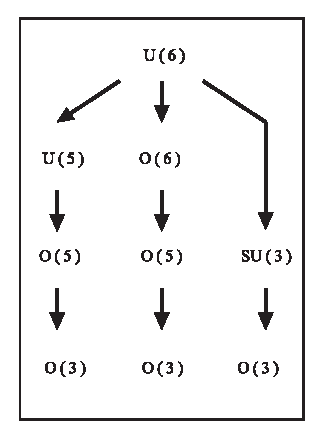
\includegraphics[scale=.65]{figure}
%
% If not, use
%\picplace{5cm}{2cm} % Give the correct figure height and width in cm
%
\caption{If the width of the figure is less than 7.8 cm use the \texttt{sidecapion} command to flush the caption on the left side of the page. If the figure is positioned at the top of the page, align the sidecaption with the top of the figure -- to achieve this you simply need to use the optional argument \texttt{[t]} with the \texttt{sidecaption} command}
\label{fig:1}       % Give a unique label
\end{figure}


\paragraph{Paragraph Heading} %
Instead of simply listing headings of different levels we recommend to let every heading be followed by at least a short passage of text. Furtheron please use the \LaTeX\ automatism for all your cross-references and citations as has already been described in Sect.~\ref{sec:2}.

Please note that the first line of text that follows a heading is not indented, whereas the first lines of all subsequent paragraphs are.

For typesetting numbered lists we recommend to use the \verb|enumerate| environment -- it will automatically render Springer's preferred layout.

\begin{enumerate}
\item{Livelihood and survival mobility are oftentimes coutcomes of uneven socioeconomic development.}
\begin{enumerate}
\item{Livelihood and survival mobility are oftentimes coutcomes of uneven socioeconomic development.}
\item{Livelihood and survival mobility are oftentimes coutcomes of uneven socioeconomic development.}
\end{enumerate}
\item{Livelihood and survival mobility are oftentimes coutcomes of uneven socioeconomic development.}
\end{enumerate}


\subparagraph{Subparagraph Heading} In order to avoid simply listing headings of different levels we recommend to let every heading be followed by at least a short passage of text. Use the \LaTeX\ automatism for all your cross-references and citations as has already been described in Sect.~\ref{sec:2}, see also Fig.~\ref{fig:2}.

Please note that the first line of text that follows a heading is not indented, whereas the first lines of all subsequent paragraphs are.

For unnumbered list we recommend to use the \verb|itemize| environment -- it will automatically render Springer's preferred layout.

\begin{itemize}
\item{Livelihood and survival mobility are oftentimes coutcomes of uneven socioeconomic development, cf. Table~\ref{tab:1}.}
\begin{itemize}
\item{Livelihood and survival mobility are oftentimes coutcomes of uneven socioeconomic development.}
\item{Livelihood and survival mobility are oftentimes coutcomes of uneven socioeconomic development.}
\end{itemize}
\item{Livelihood and survival mobility are oftentimes coutcomes of uneven socioeconomic development.}
\end{itemize}

\begin{figure}[t]
\sidecaption[t]
% Use the relevant command for your figure-insertion program
% to insert the figure file.
% For example, with the option graphics use
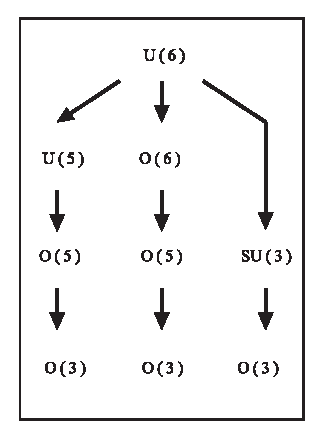
\includegraphics[scale=.65]{figure}
%
% If not, use
%\picplace{5cm}{2cm} % Give the correct figure height and width in cm
%
\caption{Please write your figure caption here}
\label{fig:2}       % Give a unique label
\end{figure}

\runinhead{Run-in Heading Boldface Version} Use the \LaTeX\ automatism for all your cross-references and citations as has already been described in Sect.~\ref{sec:2}.

\subruninhead{Run-in Heading Boldface and Italic Version} Use the \LaTeX\ automatism for all your cross-refer\-ences and citations as has already been described in Sect.~\ref{sec:2}\index{paragraph}.

\subsubruninhead{Run-in Heading Displayed Version} Use the \LaTeX\ automatism for all your cross-refer\-ences and citations as has already been described in Sect.~\ref{sec:2}\index{paragraph}.
% Use the \index{} command to code your index words
%
% For tables use
%
\begin{table}[!t]
\caption{Please write your table caption here}
\label{tab:1}       % Give a unique label
%
% For LaTeX tables use
%
\begin{tabular}{p{2cm}p{2.4cm}p{2cm}p{4.9cm}}
\hline\noalign{\smallskip}
Classes & Subclass & Length & Action Mechanism  \\
\noalign{\smallskip}\svhline\noalign{\smallskip}
Translation & mRNA$^a$  & 22 (19--25) & Translation repression, mRNA cleavage\\
Translation & mRNA cleavage & 21 & mRNA cleavage\\
Translation & mRNA  & 21--22 & mRNA cleavage\\
Translation & mRNA  & 24--26 & Histone and DNA Modification\\
\noalign{\smallskip}\hline\noalign{\smallskip}
\end{tabular}
$^a$ Table foot note (with superscript)
\end{table}
%
\section{Section Heading}
\label{sec:3}
% Always give a unique label
% and use \ref{<label>} for cross-references
% and \cite{<label>} for bibliographic references
% use \sectionmark{}
% to alter or adjust the section heading in the running head
Instead of simply listing headings of different levels we recommend to let every heading be followed by at least a short passage of text. Furtheron please use the \LaTeX\ automatism for all your cross-references and citations as has already been described in Sect.~\ref{sec:2}.

Please note that the first line of text that follows a heading is not indented, whereas the first lines of all subsequent paragraphs are.

If you want to list definitions or the like we recommend to use the Springer-enhanced \verb|description| environment -- it will automatically render Springer's preferred layout.

\begin{description}[Type 1]
\item[Type 1]{That addresses central themes pertainng to migration, health, and disease. In Sect.~\ref{sec:1}, Wilson discusses the role of human migration in infectious disease distributions and patterns.}
\item[Type 2]{That addresses central themes pertainng to migration, health, and disease. In Sect.~\ref{subsec:2}, Wilson discusses the role of human migration in infectious disease distributions and patterns.}
\end{description}

\subsection{Subsection Heading} %
In order to avoid simply listing headings of different levels we recommend to let every heading be followed by at least a short passage of text. Use the \LaTeX\ automatism for all your cross-references and citations citations as has already been described in Sect.~\ref{sec:2}.

Please note that the first line of text that follows a heading is not indented, whereas the first lines of all subsequent paragraphs are.

\begin{svgraybox}
If you want to emphasize complete paragraphs of texts we recommend to use the newly defined Springer class option \verb|graybox| and the newly defined environment \verb|svgraybox|. This will produce a 15 percent screened box 'behind' your text.

If you want to emphasize complete paragraphs of texts we recommend to use the newly defined Springer class option and environment \verb|svgraybox|. This will produce a 15 percent screened box 'behind' your text.
\end{svgraybox}


\subsubsection{Subsubsection Heading}
Instead of simply listing headings of different levels we recommend to let every heading be followed by at least a short passage of text. Furtheron please use the \LaTeX\ automatism for all your cross-references and citations as has already been described in Sect.~\ref{sec:2}.

Please note that the first line of text that follows a heading is not indented, whereas the first lines of all subsequent paragraphs are.

\begin{theorem}
Theorem text goes here.
\end{theorem}
%
% or
%
\begin{definition}
Definition text goes here.
\end{definition}

\begin{proof}
%\smartqed
Proof text goes here.
%\qed
\end{proof}

\paragraph{Paragraph Heading} %
Instead of simply listing headings of different levels we recommend to let every heading be followed by at least a short passage of text. Furtheron please use the \LaTeX\ automatism for all your cross-references and citations as has already been described in Sect.~\ref{sec:2}.

Note that the first line of text that follows a heading is not indented, whereas the first lines of all subsequent paragraphs are.
%
% For built-in environments use
%
\begin{theorem}
Theorem text goes here.
\end{theorem}
%
\begin{definition}
Definition text goes here.
\end{definition}
%
\begin{proof}
%\smartqed
Proof text goes here.
%\qed
\end{proof}
%
%
\begin{trailer}{Trailer Head}
If you want to emphasize complete paragraphs of texts in an \verb|Trailer Head| we recommend to
use  \begin{verbatim}\begin{trailer}{Trailer Head}
...
\end{trailer}\end{verbatim}
\end{trailer}
%
\begin{question}{Questions}
If you want to emphasize complete paragraphs of texts in an \verb|Questions| we recommend to
use  \begin{verbatim}\begin{question}{Questions}
...
\end{question}\end{verbatim}
\end{question}
%
%
\begin{important}{Important}
If you want to emphasize complete paragraphs of texts in an \verb|Important| we recommend to
use  \begin{verbatim}\begin{important}{Important}
...
\end{important}\end{verbatim}
\end{important}
%
\clearpage
\begin{warning}{Attention}
If you want to emphasize complete paragraphs of texts in an \verb|Attention| we recommend to
use  \begin{verbatim}\begin{warning}{Attention}
...
\end{warning}\end{verbatim}
\end{warning}

\begin{programcode}{Program Code}
If you want to emphasize complete paragraphs of texts in an \verb|Program Code| we recommend to
use

\verb|\begin{programcode}{Program Code}|

\verb|\begin{verbatim}...\end{verbatim}|

\verb|\end{programcode}|

\end{programcode}
%
\begin{tips}{Tips}
If you want to emphasize complete paragraphs of texts in an \verb|Tips| we recommend to
use  \begin{verbatim}\begin{tips}{Tips}
...
\end{tips}\end{verbatim}
\end{tips}
%
%
\begin{overview}{Overview}
If you want to emphasize complete paragraphs of texts in an \verb|Overview| we recommend to
use  \begin{verbatim}\begin{overview}{Overview}
...
\end{overview}\end{verbatim}
\end{overview}
\clearpage
\begin{backgroundinformation}{Background Information}
If you want to emphasize complete paragraphs of texts in an \verb|Background|
\verb|Information| we recommend to
use

\verb|\begin{backgroundinformation}{Background Information}|

\verb|...|

\verb|\end{backgroundinformation}|
\end{backgroundinformation}
\begin{legaltext}{Legal Text}
If you want to emphasize complete paragraphs of texts in an \verb|Legal Text| we recommend to
use  \begin{verbatim}\begin{legaltext}{Legal Text}
...
\end{legaltext}\end{verbatim}
\end{legaltext}
%
\begin{acknowledgement}
If you want to include acknowledgments of assistance and the like at the end of an individual chapter please use the \verb|acknowledgement| environment -- it will automatically render Springer's preferred layout.
\end{acknowledgement}
%
\section*{Appendix}
\addcontentsline{toc}{section}{Appendix}
%
When placed at the end of a chapter or contribution (as opposed to at the end of the book), the numbering of tables, figures, and equations in the appendix section continues on from that in the main text. Hence please \textit{do not} use the \verb|appendix| command when writing an appendix at the end of your chapter or contribution. If there is only one the appendix is designated ``Appendix'', or ``Appendix 1'', or ``Appendix 2'', etc. if there is more than one.

\begin{equation}
a \times b = c
\end{equation}
% Problems or Exercises should be sorted chapterwise
\section*{Problems}
\addcontentsline{toc}{section}{Problems}
%
% Use the following environment.
% Don't forget to label each problem;
% the label is needed for the solutions' environment
\begin{prob}
\label{prob1}
A given problem or Excercise is described here. The
problem is described here. The problem is described here.
\end{prob}

\begin{prob}
\label{prob2}
\textbf{Problem Heading}\\
(a) The first part of the problem is described here.\\
(b) The second part of the problem is described here.
\end{prob}

%%%%%%%%%%%%%%%%%%%%%%%% referenc.tex %%%%%%%%%%%%%%%%%%%%%%%%%%%%%%
% sample references
% %
% Use this file as a template for your own input.
%
%%%%%%%%%%%%%%%%%%%%%%%% Springer-Verlag %%%%%%%%%%%%%%%%%%%%%%%%%%
%
% BibTeX users please use
% \bibliographystyle{}
% \bibliography{}
%


\biblstarthook{In view of the parallel print and (chapter-wise) online publication of your book at \url{www.springerlink.com} it has been decided that -- as a genreral rule --  references should be sorted chapter-wise and placed at the end of the individual chapters. However, upon agreement with your contact at Springer you may list your references in a single seperate chapter at the end of your book. Deactivate the class option \texttt{sectrefs} and the \texttt{thebibliography} environment will be put out as a chapter of its own.\\\indent
References may be \textit{cited} in the text either by number (preferred) or by author/year.\footnote{Make sure that all references from the list are cited in the text. Those not cited should be moved to a separate \textit{Further Reading} section or chapter.} If the citatiion in the text is numbered, the reference list should be arranged in ascending order. If the citation in the text is author/year, the reference list should be \textit{sorted} alphabetically and if there are several works by the same author, the following order should be used:
\begin{enumerate}
\item all works by the author alone, ordered chronologically by year of publication
\item all works by the author with a coauthor, ordered alphabetically by coauthor
\item all works by the author with several coauthors, ordered chronologically by year of publication.
\end{enumerate}
The \textit{styling} of references\footnote{Always use the standard abbreviation of a journal's name according to the ISSN \textit{List of Title Word Abbreviations}, see \url{http://www.issn.org/en/node/344}} depends on the subject of your book:
\begin{itemize}
\item The \textit{two} recommended styles for references in books on \textit{mathematical, physical, statistical and computer sciences} are depicted in ~\cite{science-contrib, science-online, science-mono, science-journal, science-DOI} and ~\cite{phys-online, phys-mono, phys-journal, phys-DOI, phys-contrib}.
\item Examples of the most commonly used reference style in books on \textit{Psychology, Social Sciences} are~\cite{psysoc-mono, psysoc-online,psysoc-journal, psysoc-contrib, psysoc-DOI}.
\item Examples for references in books on \textit{Humanities, Linguistics, Philosophy} are~\cite{humlinphil-journal, humlinphil-contrib, humlinphil-mono, humlinphil-online, humlinphil-DOI}.
\item Examples of the basic Springer style used in publications on a wide range of subjects such as \textit{Computer Science, Economics, Engineering, Geosciences, Life Sciences, Medicine, Biomedicine} are ~\cite{basic-contrib, basic-online, basic-journal, basic-DOI, basic-mono}. 
\end{itemize}
}

\begin{thebibliography}{99.}%
% and use \bibitem to create references.
%
% Use the following syntax and markup for your references if 
% the subject of your book is from the field 
% "Mathematics, Physics, Statistics, Computer Science"
%
% Contribution 
\bibitem{science-contrib} Broy, M.: Software engineering --- from auxiliary to key technologies. In: Broy, M., Dener, E. (eds.) Software Pioneers, pp. 10-13. Springer, Heidelberg (2002)
%
% Online Document
\bibitem{science-online} Dod, J.: Effective substances. In: The Dictionary of Substances and Their Effects. Royal Society of Chemistry (1999) Available via DIALOG. \\
\url{http://www.rsc.org/dose/title of subordinate document. Cited 15 Jan 1999}
%
% Monograph
\bibitem{science-mono} Geddes, K.O., Czapor, S.R., Labahn, G.: Algorithms for Computer Algebra. Kluwer, Boston (1992) 
%
% Journal article
\bibitem{science-journal} Hamburger, C.: Quasimonotonicity, regularity and duality for nonlinear systems of partial differential equations. Ann. Mat. Pura. Appl. \textbf{169}, 321--354 (1995)
%
% Journal article by DOI
\bibitem{science-DOI} Slifka, M.K., Whitton, J.L.: Clinical implications of dysregulated cytokine production. J. Mol. Med. (2000) doi: 10.1007/s001090000086 
%
\bigskip

% Use the following (APS) syntax and markup for your references if 
% the subject of your book is from the field 
% "Mathematics, Physics, Statistics, Computer Science"
%
% Online Document
\bibitem{phys-online} J. Dod, in \textit{The Dictionary of Substances and Their Effects}, Royal Society of Chemistry. (Available via DIALOG, 1999), 
\url{http://www.rsc.org/dose/title of subordinate document. Cited 15 Jan 1999}
%
% Monograph

\bibitem{phys-mono} H. Ibach, H. L\"uth, \textit{Solid-State Physics}, 2nd edn. (Springer, New York, 1996), pp. 45-56 
%
% Journal article
\bibitem{phys-journal} S. Preuss, A. Demchuk Jr., M. Stuke, Appl. Phys. A \textbf{61}
%
% Journal article by DOI
\bibitem{phys-DOI} M.K. Slifka, J.L. Whitton, J. Mol. Med., doi: 10.1007/s001090000086
%
% Contribution 
\bibitem{phys-contrib} S.E. Smith, in \textit{Neuromuscular Junction}, ed. by E. Zaimis. Handbook of Experimental Pharmacology, vol 42 (Springer, Heidelberg, 1976), p. 593
%
\bigskip
%
% Use the following syntax and markup for your references if 
% the subject of your book is from the field 
% "Psychology, Social Sciences"
%
%
% Monograph
\bibitem{psysoc-mono} Calfee, R.~C., \& Valencia, R.~R. (1991). \textit{APA guide to preparing manuscripts for journal publication.} Washington, DC: American Psychological Association.
%
% Online Document
\bibitem{psysoc-online} Dod, J. (1999). Effective substances. In: The dictionary of substances and their effects. Royal Society of Chemistry. Available via DIALOG. \\
\url{http://www.rsc.org/dose/Effective substances.} Cited 15 Jan 1999.
%
% Journal article
\bibitem{psysoc-journal} Harris, M., Karper, E., Stacks, G., Hoffman, D., DeNiro, R., Cruz, P., et al. (2001). Writing labs and the Hollywood connection. \textit{J Film} Writing, 44(3), 213--245.
%
% Contribution 
\bibitem{psysoc-contrib} O'Neil, J.~M., \& Egan, J. (1992). Men's and women's gender role journeys: Metaphor for healing, transition, and transformation. In B.~R. Wainrig (Ed.), \textit{Gender issues across the life cycle} (pp. 107--123). New York: Springer.
%
% Journal article by DOI
\bibitem{psysoc-DOI}Kreger, M., Brindis, C.D., Manuel, D.M., Sassoubre, L. (2007). Lessons learned in systems change initiatives: benchmarks and indicators. \textit{American Journal of Community Psychology}, doi: 10.1007/s10464-007-9108-14.
%
%
% Use the following syntax and markup for your references if 
% the subject of your book is from the field 
% "Humanities, Linguistics, Philosophy"
%
\bigskip
%
% Journal article
\bibitem{humlinphil-journal} Alber John, Daniel C. O'Connell, and Sabine Kowal. 2002. Personal perspective in TV interviews. \textit{Pragmatics} 12:257--271
%
% Contribution 
\bibitem{humlinphil-contrib} Cameron, Deborah. 1997. Theoretical debates in feminist linguistics: Questions of sex and gender. In \textit{Gender and discourse}, ed. Ruth Wodak, 99--119. London: Sage Publications.
%
% Monograph
\bibitem{humlinphil-mono} Cameron, Deborah. 1985. \textit{Feminism and linguistic theory.} New York: St. Martin's Press.
\bibitem{albertohonor} Calderón, Alberto, F. M. Christ, Carlos E. Kenig and Cora Sadosky. “Harmonic analysis and partial differential equations : essays in honor of Alberto P. Calderón.” (1999).
%
% Online Document
\bibitem{humlinphil-online} Dod, Jake. 1999. Effective substances. In: The dictionary of substances and their effects. Royal Society of Chemistry. Available via DIALOG. \\
http://www.rsc.org/dose/title of subordinate document. Cited 15 Jan 1999
%
% Journal article by DOI
\bibitem{humlinphil-DOI} Suleiman, Camelia, Daniel C. O'Connell, and Sabine Kowal. 2002. `If you and I, if we, in this later day, lose that sacred fire...': Perspective in political interviews. \textit{Journal of Psycholinguistic Research}. doi: 10.1023/A:1015592129296.
%
%
%
\bigskip
%
%
% Use the following syntax and markup for your references if 
% the subject of your book is from the field 
% "Computer Science, Economics, Engineering, Geosciences, Life Sciences"
%
%
% Contribution 
\bibitem{basic-contrib} Brown B, Aaron M (2001) The politics of nature. In: Smith J (ed) The rise of modern genomics, 3rd edn. Wiley, New York 
%
% Online Document
\bibitem{basic-online} Dod J (1999) Effective Substances. In: The dictionary of substances and their effects. Royal Society of Chemistry. Available via DIALOG. \\
\url{http://www.rsc.org/dose/title of subordinate document. Cited 15 Jan 1999}
%
% Journal article by DOI
\bibitem{basic-DOI} Slifka MK, Whitton JL (2000) Clinical implications of dysregulated cytokine production. J Mol Med, doi: 10.1007/s001090000086
%
% Journal article
\bibitem{basic-journal} Smith J, Jones M Jr, Houghton L et al (1999) Future of health insurance. N Engl J Med 965:325--329
%
% Monograph
\bibitem{basic-mono} South J, Blass B (2001) The future of modern genomics. Blackwell, London 
%
\end{thebibliography}


%%%%%%%%%%%%%%%%%%%%%part.tex%%%%%%%%%%%%%%%%%%%%%%%%%%%%%%%%%%
% 
% sample part title
%
% Use this file as a template for your own input.
%
%%%%%%%%%%%%%%%%%%%%%%%% Springer %%%%%%%%%%%%%%%%%%%%%%%%%%

\begin{partbacktext}
\part{(The Elements of Lebesgue Measure)}

\end{partbacktext}
%%%%%%%%%%%%%%%%%%%%% appendix.tex %%%%%%%%%%%%%%%%%%%%%%%%%%%%%%%%%
%
% sample appendix
%
% Use this file as a template for your own input.
%
%%%%%%%%%%%%%%%%%%%%%%%% Springer-Verlag %%%%%%%%%%%%%%%%%%%%%%%%%%

\appendix
\motto{All's well that ends well}
\chapter{Chapter Heading}
\label{introA} % Always give a unique label
% use \chaptermark{}
% to alter or adjust the chapter heading in the running head

Use the template \emph{appendix.tex} together with the Springer document class SVMono (monograph-type books) or SVMult (edited books) to style appendix of your book.


\section{Section Heading}
\label{sec:A1}
% Always give a unique label
% and use \ref{<label>} for cross-references
% and \cite{<label>} for bibliographic references
% use \sectionmark{}
% to alter or adjust the section heading in the running head
Instead of simply listing headings of different levels we recommend to let every heading be followed by at least a short passage of text. Furtheron please use the \LaTeX\ automatism for all your cross-references and citations.


\subsection{Subsection Heading}
\label{sec:A2}
Instead of simply listing headings of different levels we recommend to let every heading be followed by at least a short passage of text. Furtheron please use the \LaTeX\ automatism for all your cross-references and citations as has already been described in Sect.~\ref{sec:A1}.

For multiline equations we recommend to use the \verb|eqnarray| environment.
\begin{eqnarray}
\vec{a}\times\vec{b}=\vec{c} \nonumber\\
\vec{a}\times\vec{b}=\vec{c}
\label{eq:A01}
\end{eqnarray}

\subsubsection{Subsubsection Heading}
Instead of simply listing headings of different levels we recommend to let every heading be followed by at least a short passage of text. Furtheron please use the \LaTeX\ automatism for all your cross-references and citations as has already been described in Sect.~\ref{sec:A2}.

Please note that the first line of text that follows a heading is not indented, whereas the first lines of all subsequent paragraphs are.

% For figures use
%
\begin{figure}[t]
\sidecaption[t]
%\centering
% Use the relevant command for your figure-insertion program
% to insert the figure file.
% For example, with the option graphics use
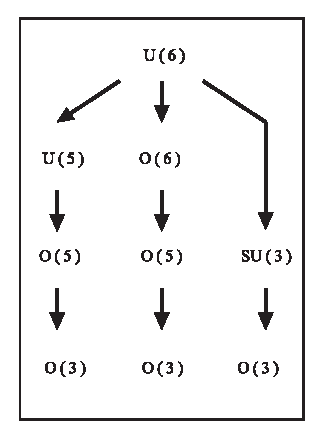
\includegraphics[scale=.65]{figure}
%
% If not, use
%\picplace{5cm}{2cm} % Give the correct figure height and width in cm
%
\caption{Please write your figure caption here}
\label{fig:A1}       % Give a unique label
\end{figure}

% For tables use
%
\begin{table}
\caption{Please write your table caption here}
\label{tab:A1}       % Give a unique label
%
% For LaTeX tables use
%
\begin{tabular}{p{2cm}p{2.4cm}p{2cm}p{4.9cm}}
\hline\noalign{\smallskip}
Classes & Subclass & Length & Action Mechanism  \\
\noalign{\smallskip}\hline\noalign{\smallskip}
Translation & mRNA$^a$  & 22 (19--25) & Translation repression, mRNA cleavage\\
Translation & mRNA cleavage & 21 & mRNA cleavage\\
Translation & mRNA  & 21--22 & mRNA cleavage\\
Translation & mRNA  & 24--26 & Histone and DNA Modification\\
\noalign{\smallskip}\hline\noalign{\smallskip}
\end{tabular}
$^a$ Table foot note (with superscript)
\end{table}
%


\backmatter%%%%%%%%%%%%%%%%%%%%%%%%%%%%%%%%%%%%%%%%%%%%%%%%%%%%%%%
%%%%%%%%%%%%%%%%%%%%%%acronym.tex%%%%%%%%%%%%%%%%%%%%%%%%%%%%%%%%%%%%%%%%%
% sample list of acronyms
%
% Use this file as a template for your own input.
%
%%%%%%%%%%%%%%%%%%%%%%%% Springer %%%%%%%%%%%%%%%%%%%%%%%%%%

\Extrachap{Acronyms and Abbreviations}
Here you can see a list of important acronyms.
\begin{description}[list]
\setlength{\labelwidth}{6em}
\item[ANSI]{\href{https://www.ansi.org/}{American National Standards Institute}}
\item[ASCII]{American Standard Code for Information Interchange}
\item[CPU]{Central Processing Unit}
\item[CUDA]{Compute Unified Device Architecture}
\item[DRAM]{Dynamic Random Access Memory}
\item[GNU]{GNU's Not Unix}
\item[GPU]{Graphics Processing Unit}
\item[grep]{g lobal(ly) search r egular e xpression p rint}
\item[NVRAM]{Non-Volatile Random Access Memory}
\item[pip]{Pip Installs Packages}
\item[RAM]{Random Access Memory}
\item[SDRAM]{Static Random Access Memory} 
\item[TPU]{Tensor Processing Unit}

\end{description}
%%%%%%%%%%%%%%%%%%%%%%acronym.tex%%%%%%%%%%%%%%%%%%%%%%%%%%%%%%%%%%%%%%%%%
% sample list of acronyms
%
% Use this file as a template for your own input.
%
%%%%%%%%%%%%%%%%%%%%%%%% Springer %%%%%%%%%%%%%%%%%%%%%%%%%%

\Extrachap{Glossary}


Use the template \emph{glossary.tex} together with the Springer document class SVMono (monograph-type books) or SVMult (edited books) to style your glossary\index{glossary} in the Springer layout.


\runinhead{GNU} GNU is not UNIX 

\runinhead{glossary term} Write here the description of the glossary term. Write here the description of the glossary term. Write here the description of the glossary term.

\runinhead{glossary term} Write here the description of the glossary term. Write here the description of the glossary term. Write here the description of the glossary term.

\runinhead{abs} datenwise

\runinhead{glossary term} Write here the description of the glossary term. Write here the description of the glossary term. Write here the description of the glossary term.
\bibliographystyle{alpha}
\bibliography{references.bib}

\Extrachap{Solutions}

\section*{Problems of Chapter~\ref{intro}}

\begin{sol}{prob1}
The solution\index{problems}\index{solutions} is revealed here.
\end{sol}


\begin{sol}{prob2}
\textbf{Problem Heading}\\
(a) The solution of first part is revealed here.\\
(b) The solution of second part is revealed here.
\end{sol}


\printindex

%%%%%%%%%%%%%%%%%%%%%%%%%%%%%%%%%%%%%%%%%%%%%%%%%%%%%%%%%%%%%%%%%%%%%%

\end{document}





